%%
%% IVP 2026 report template
%%
\documentclass[a4paper,fleqn]{cas-sc}

\usepackage[authoryear]{natbib}

\usepackage{float}
\usepackage{amsmath}
\usepackage{booktabs}
\usepackage{graphicx}
\usepackage{multirow}

%%%Author definitions
\def\tsc#1{\csdef{#1}{\textsc{\lowercase{#1}}\xspace}}

\begin{document}

\graphicspath{{./}}

% Change your group name in both by replacing X!
\shorttitle{Group 'A buisness of ferrets'}
\shortauthors{Group 'A buisness of ferrets'}

% Change your group name in both by replacing X!
\title [mode = title]{IVP2026 Group 'A buisness of ferrets' Report}

% Change your names here for all members
% Replace StudentNameX with your full name. You can use spaces here.
% Replace studentidX with your student id. Only the digits. Do not put i or I at the beginning!
% Replace kaggleidX with your Kaggle handle and gitnameX with your Git username.
% Do not omit any optional fields
% Order of authors should be in alphebetical ordered by last name.
\author[1]{David Weis}[studentid=studentid1, kaggleid=kaggleid1, gitname=gitname1]
\author[1]{Linn Maleen Schulze}[studentid=i6414209, kaggleid=linnmaleenschulze, gitname=linn-maleen]
\author[1]{Mihai Solescu}[studentid=studentid3, kaggleid=kaggleid3, gitname=gitname3]

% Do not change!
\affiliation[1]{organization={Department of Advanced Computing Sciences, Maastricht University},
            city={Maastricht},
            country={The Netherlands}}

% Do not change!!
\begin{abstract}
This report has been submitted for the BCS2710A - Image and Video Processing course in Department of Advanced Computing Sciences at Maastricht University. The report is a requirement of the IVP-2026 challenge. The challenge has been created by Dr.\@~Petra Bosilj \citep{the_challenge}.
\end{abstract}

% Do not change!!
\begin{keywords}
BCS2710A \sep IVP2026 \sep Digital images \sep Analogue clock reader 
\end{keywords}
\maketitle 
\clearpage

% Your main text goes here!!!!
\section{Methodology}
Explain only your methodology using properly referenced papers, algorithms, models and justifications.

You do not need to present your results or explain the problem presented to you through the challenge.


\bibliographystyle{cas-model2-names}
\bibliography{references}

\begin{figure}[h]
    \centering
    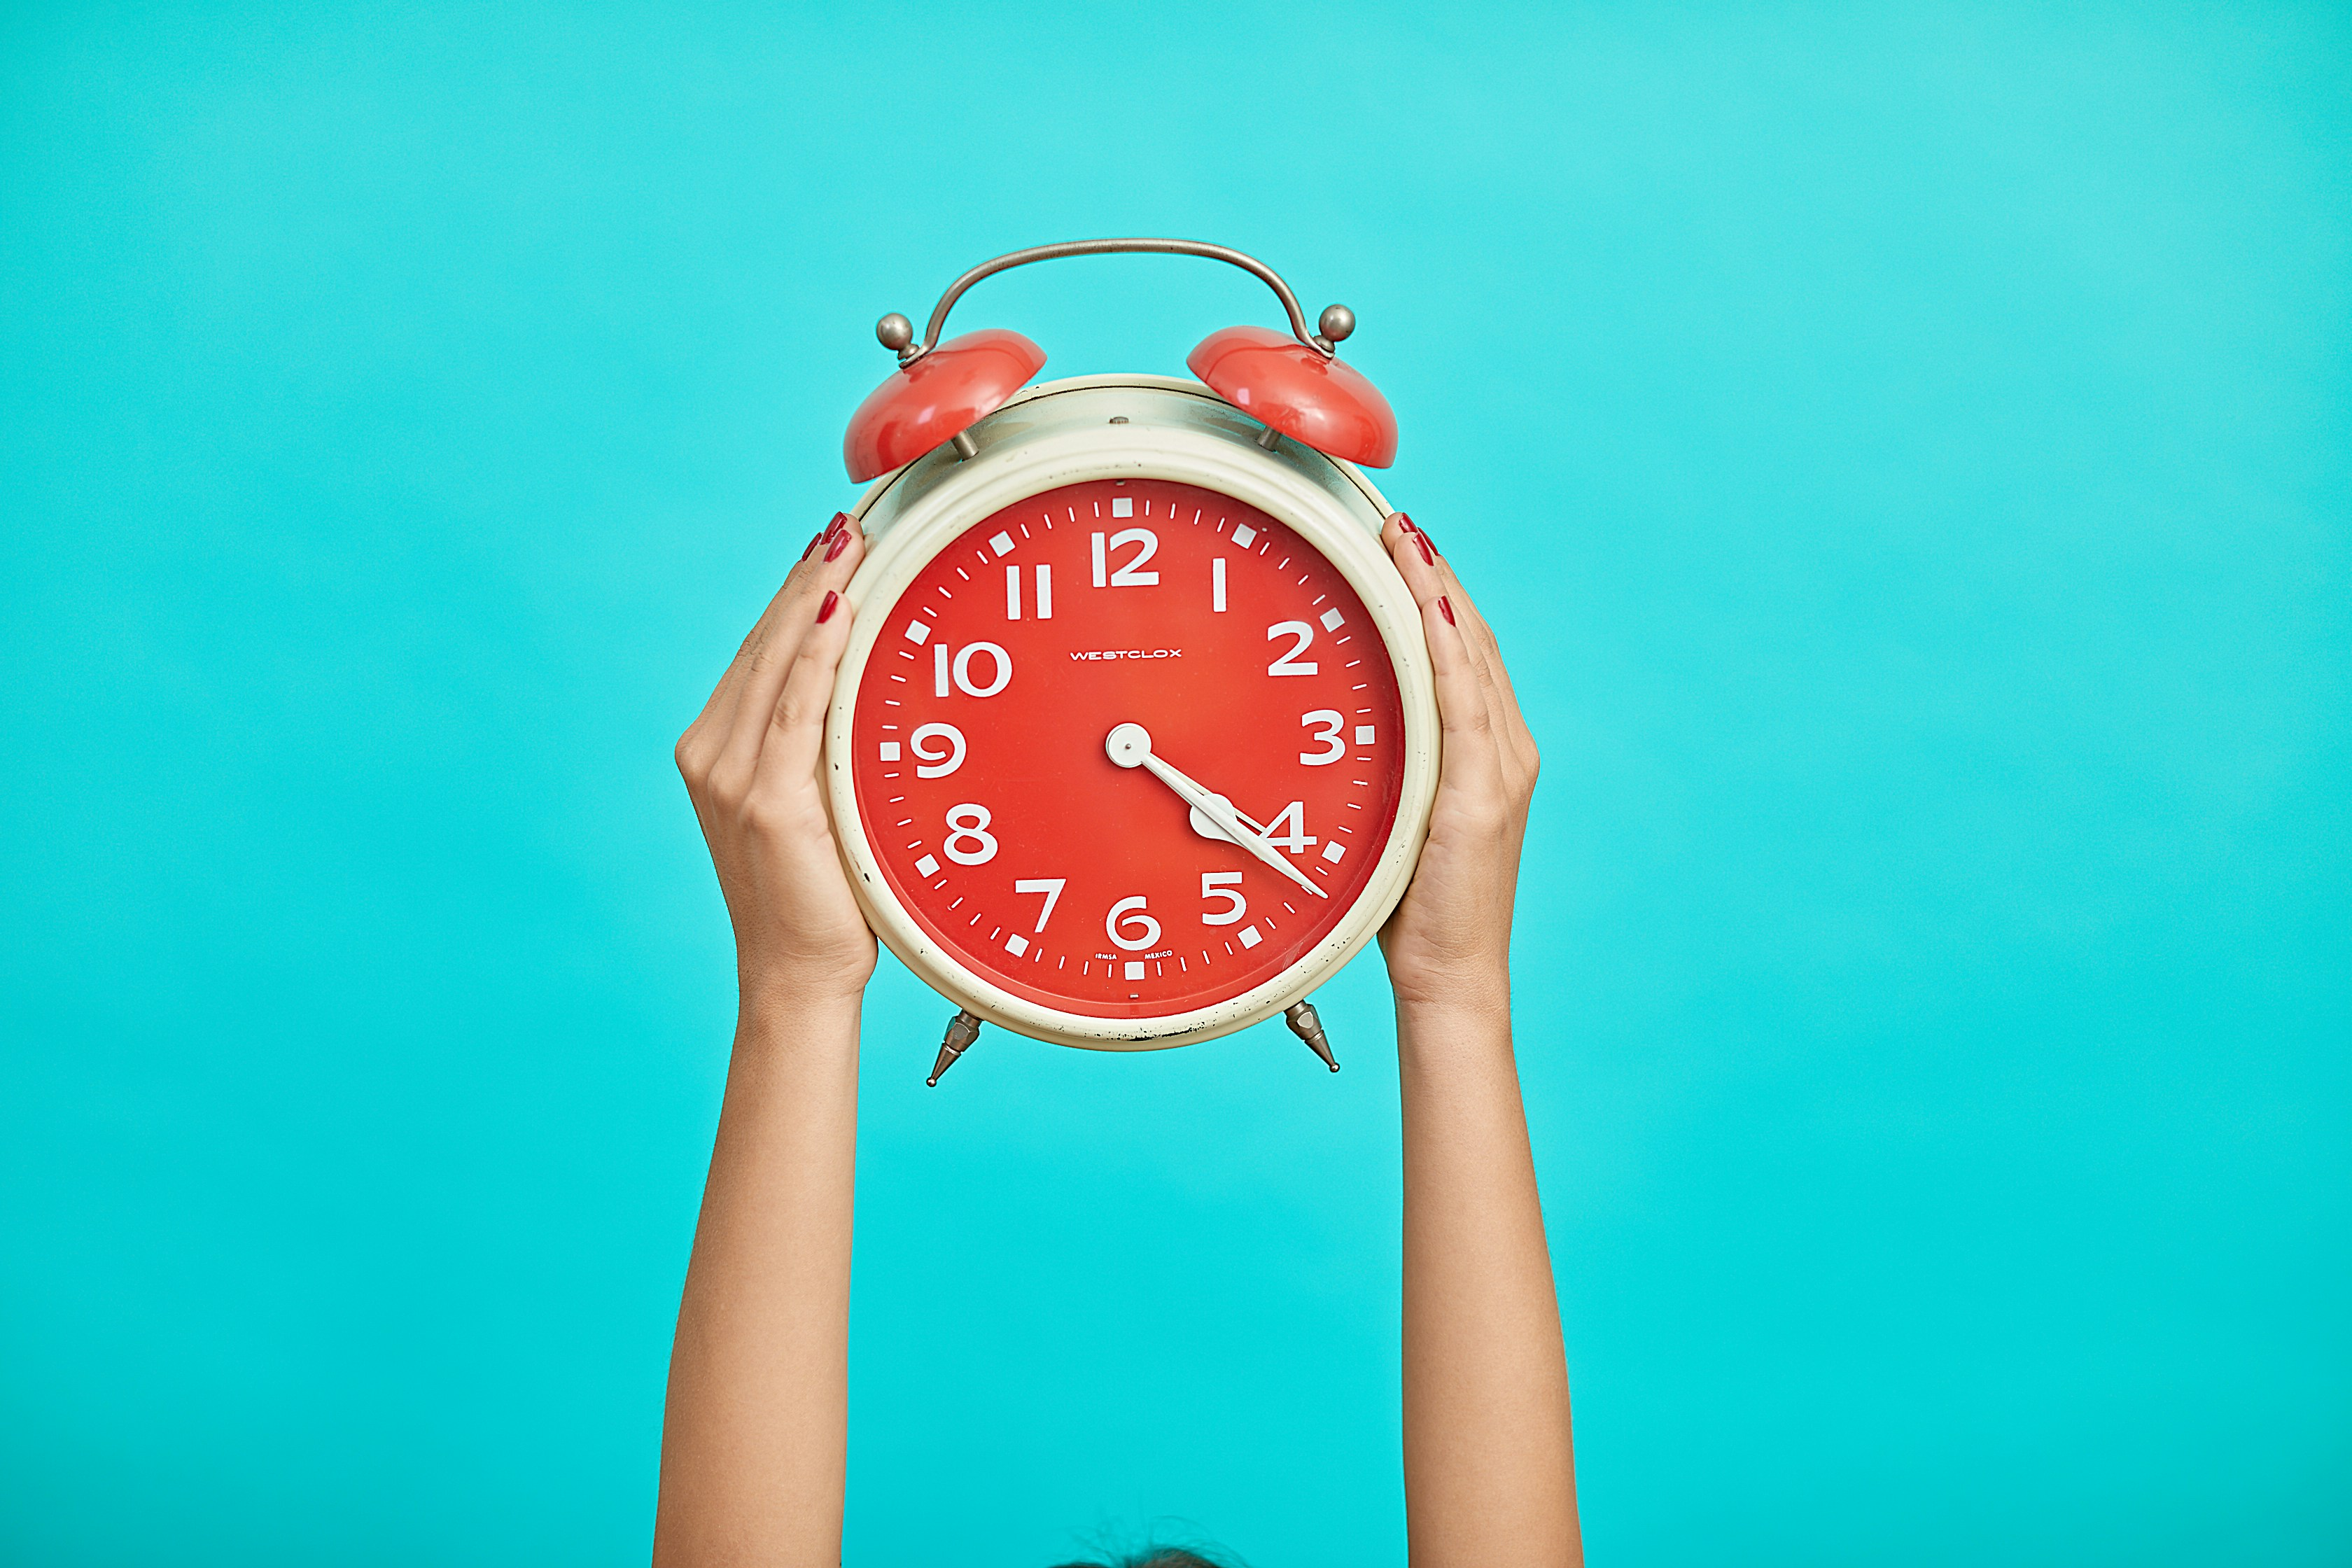
\includegraphics[height=150px]{Images/malvestida-unsplash.jpg}
    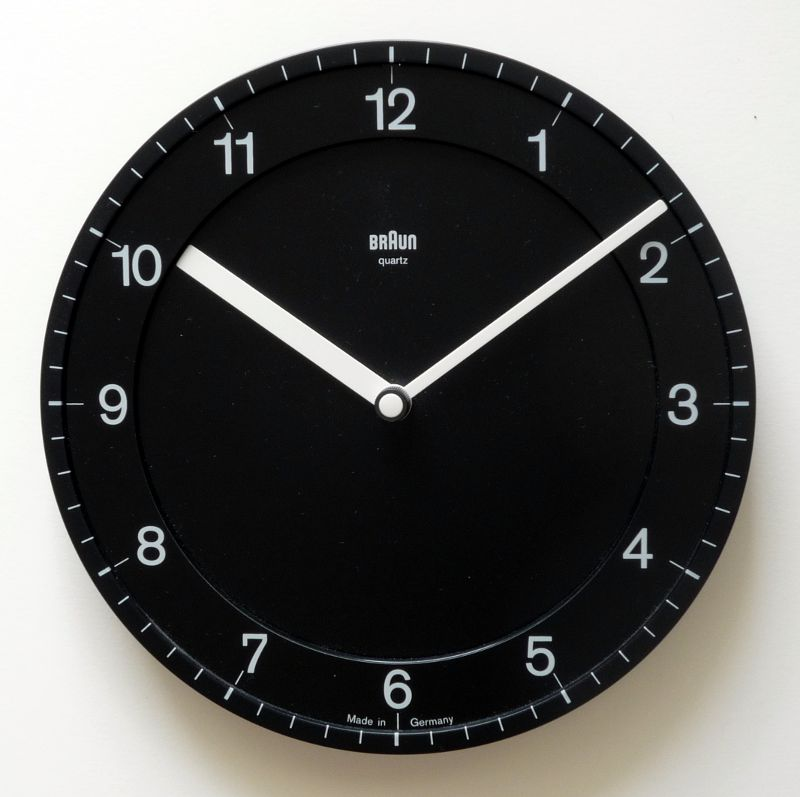
\includegraphics[height=150px]{Images/Phrontis-commons_wikimedia_org-braun-abw30-black.jpg}
    \caption{Example figure. Left: photo by malvestida from \url{unsplash.com}. Right: photo by Phrontis from \url{commons.wikimedia.org}, licensed under \href{https://creativecommons.org/licenses/by-sa/3.0/}{CC BY-SA 3.0}.}
    \label{fig:image1}
\end{figure}
\begin{figure}[h]
    \centering
    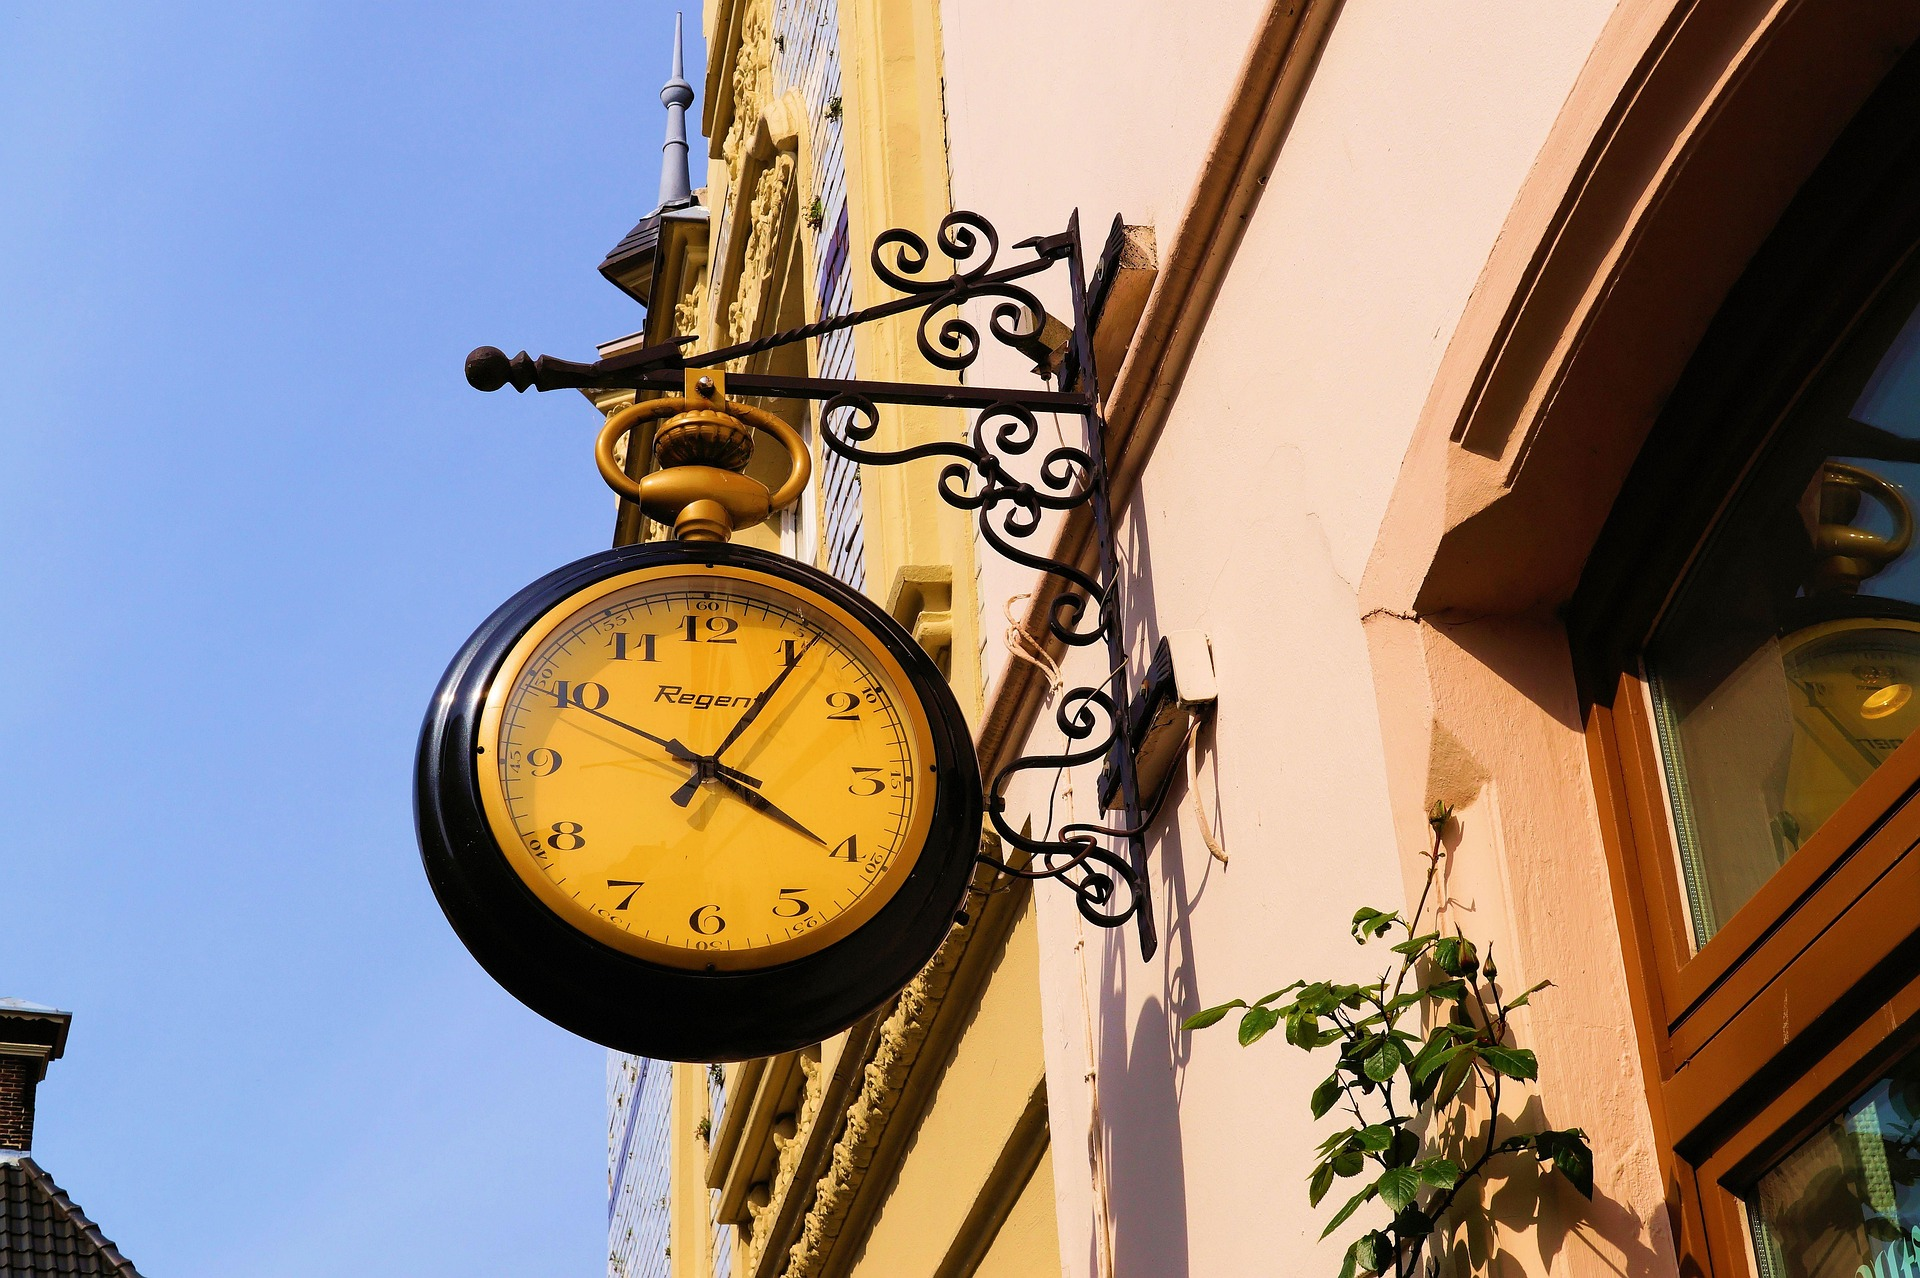
\includegraphics[width=0.4\linewidth]{Images/kapa65-pixabay.jpg}
    \caption{Second example figure. Photo by kapa65 from \url{pixabay.com}.}
    \label{fig:image2}
\end{figure}

\end{document}
